\documentclass[11pt,a4paper]{ctexart}

% 页面设置
\usepackage{geometry}
\geometry{left=2cm,right=2cm,top=2.8cm,bottom=2.8cm}

% 数学与排版
\usepackage{amsmath,amssymb}   % 数学公式
\usepackage{enumitem}          % 题号列表控制
\usepackage{fancyhdr}          % 页脚设置
\usepackage{tasks}             % 选择题横排
\usepackage{graphicx}          % 处理图片
\usepackage{hyperref}          % 目录跳转
\usepackage{lastpage}          % 获取总页数
\usepackage{tikz,times}        % 绘图宏包、字体宏包
\usepackage{tikz-3dplot}       % 三维图形宏包
\usetikzlibrary{3d,calc}       % 3d绘图及计算需要的库
\hypersetup{
    colorlinks=true,    % 目录链接带颜色
    linkcolor=black,    % 链接颜色为黑色（不刺眼）
    pdfstartview=FitH,  % PDF打开时适配页面宽度
}

% ===== tasks宏包核心配置 =====
\settasks{
    label=(\arabic*), % 选项标签
    label-align = left,        % 标签左对齐（适配(A)格式）
    label-width = 2em,         % 标签宽度
    item-indent = 3em,         % 选项内容缩进（和标签宽度一致）
    column-sep = 1.5em,        % 选项列间距
    after-item-skip = 0pt,     % 取消选项间垂直间距（避免竖排）
    before-skip = 0.5em,       % 选项和题干间的小间距
    after-skip = 0.8em,        % 选项和下一题间的间距
} 
% =========================

% ======= 页脚设置 ==========
\pagestyle{fancy} % 启用fancy页眉页脚样式
\fancyhf{} % 清空默认的页眉页脚内容
\renewcommand{\headrulewidth}{0pt} % 删除页眉上方横线
\renewcommand{\footrulewidth}{0pt} % 删除页脚上方横线
\fancyfootoffset{0pt} % 页脚左右对齐页面边界
\renewcommand{\footnoterule}{} % 取消脚注横线（避免冲突）
\fancyfoot[R]{\small \thepage}
% =========================

% 题型标题样式 （如选择题，填空题，解答题）
\newcommand{\sectiontitle}[1]{
  \par\noindent\textbf{#1}\par% 顶格、加粗、独立段落
  }

% 1-21题号格式 
\setlist[enumerate,1]{
    label=\arabic*.\ ,
    itemsep=0.6em,   % 行间距
    parsep=0.6em,    % 题干内换行间距（匹配\\[0.6em]）
    before=\setlength{\baselineskip}{1.5\baselineskip}
    }

%页码设置
\newcounter{chapPage}
\AddToHook{shipout/after}{\stepcounter{chapPage}}

\begin{document}

% ===================== 封面 =====================
\thispagestyle{empty}
\begin{center}
    \vspace*{\fill}% 垂直居中
    {\Huge\bfseries 知己知彼}\\[1.5cm]% 标题
    {\Large LJR}\\[0.5cm]% 署名
    \vspace*{\fill}
\end{center}
\newpage

% ===================== 目录页 =====================
\tableofcontents % 生成目录
\newpage 

% ================ 知己知彼pi ===================
\clearpage %新的一页
\setcounter{enumi}{0}   % 卷II选择题号从1开始
\phantomsection
\addcontentsline{toc}{section}{\texorpdfstring{知己知彼$\pi$}{知己知彼pi}} % 加入目录
\setcounter{chapPage}{1} %初始化页数
\fancyfoot[C]{\small 高三数学\ 第 \thechapPage 页 (共$6$页)} %居中页脚

\begin{center} 
    {\LARGE \textbf{知己知彼$\pi$}}\\[1em]
\end{center}

\sectiontitle{一、选择题共 $10$ 小题，每小题 $4$ 分，共 $40$ 分。在每小题的四个选项中，选出符合题目要求的一项。}

\begin{enumerate}

    \item 集合$A=\{x \mid -1 \le x \le 1\ \}$,集合$B=\{x\mid a-1\le x \le 2a-1\ \}$，若$B \subseteq A$,则
    \begin{tasks}(4)
        \task $a<1$ 
        \task $a \le 1$
        \task $0 \le a \le 1$
        \task $0 < a \le 1$
    \end{tasks}

    \item 若$z \cdot \overline{z}+2=2z $，则$z=$
    \begin{tasks}(4)
        \task $1+i$ 
        \task $1-i$
        \task $-1+i$
        \task $-1-i$
    \end{tasks}

    \item “$a \le 0 $”是“$f(x)= \mid (ax-1)x \mid $在$(\ 0, + \infty \ )$内单调递增”的
    \begin{enumerate}[label=(\Alph*)]
        \item 充分不必要条件
        \item 必要不充分条件
        \item 充要条件
        \item 既不充分也不必要条件
    \end{enumerate}

    \item $f(x)= \cos 2x+ \cos 3x\ ,x \in (\ 0,\pi \ )$，若$f(x)$有两个零点$x_1,x_2(\ x_1<x_2\ )$，则
    \begin{tasks}(2)
        \task $\dfrac{2\pi }{5} \in \{x_1,x_2\}$ 
        \task $x_2=2x_1$
        \task $\cos x_1+ \cos x_2=\dfrac{1}{2}$
        \task $\cos x_1 \cos x_2=\dfrac{\sqrt{2}}{2}$
    \end{tasks}
    
    \item $O$为坐标原点，过$y=2px\ (p>0)$焦点的直线$l$与该抛物线交与$A,B$两点，若$\mid AB \mid =12\ ,\ S_{\triangle OAB}=4\sqrt{6}$，则$p=$
    \begin{tasks}(4)
        \task $4$ 
        \task $3$
        \task $2 \sqrt{6}$
        \task $3 \sqrt{2}$
    \end{tasks}
    \newpage

    \item 已知$a=-\ln \dfrac{1}{9}\ ,\ b=0.1e^{0.1}\ ,\ c=\dfrac{1}{9}$，则
    \begin{tasks}(4)
        \task $a<c<b$ 
        \task $c<a<b$
        \task $a<b<c$
        \task $b<a<c$
    \end{tasks}

    \item 已知$O$是$\triangle ABC$所在平面内的一点，且$\mid \overrightarrow{AB} \mid=2\ ,\ \ \overrightarrow{OA} \cdot \overrightarrow{AC}=-1\ ,\ \overrightarrow{OC} \cdot \overrightarrow{AC}=1$，则$\angle ABC$最大值为
    \begin{tasks}(4)
        \task $\dfrac{\pi}{6}$ 
        \task $\dfrac{\pi}{4}$
        \task $\dfrac{\pi}{3}$
        \task $\dfrac{\pi}{2}$
    \end{tasks}
    

    \item 从重量为$1,2,\ldots\ ,10$的砝码（每种各两个）中选出若干个，使其总质量恰为$9g$方法总数为$m$，下列展开式中$x^9$系数为$m$的是
    \begin{tasks}(2)
        \task $(1+x)(1+x^2) \cdots (1+x^{10})$
        \task $(1+x)(1+2x) \cdots (1+10x)$
        \task $(1+x)(1+x^2)^2 \cdots (1+x^{10})^{10}$ 
        \task $(1+x)^2(1+x+x^2)^2 \cdots (1+x+ \cdots +x^{10})^2$ 
    \end{tasks}

    \item 定义在$(\ 0,+\infty \ )$的函数$f(x)$满足$f(\dfrac{x}{y})=yf(x)-xf(y)$，且当$x>1$时，$f(x)>0$，则    
    \begin{tasks}(2)
        \task $f(x^2) \ge 2f(x)$ 
        \task $f(x^3)f(x) \ge 2f^2(x^2)$
        \task $f(x^2) \le 2f(x)$
        \task $f(x^3)f(x) \le 2f^2(x^2)$
    \end{tasks}

    \item 三棱锥$P-ABC$ 中，$AB=2\sqrt{2}$ ，$PC=1$， $PA+PB=4$，$CA-CB=2$，且$PC \perp AB$，则二面角$P-AB-C$余弦值最小为
    \begin{tasks}(4)
        \task $\dfrac{\sqrt{2}}{3}$ 
        \task $\dfrac{3}{4}$
        \task $\dfrac{1}{2}$
        \task $\dfrac{\sqrt{10}}{5}$
    \end{tasks}
\end{enumerate}

\newpage
\sectiontitle{二、填空题。共5小题，每小题5分，共25分。}
\begin{enumerate}[start=11] % 填空题从11开始编号

    \item 有八张卡片$1,2,\ldots\,8$，现从中随机抽$3$张，抽出$3$张数字之和与未抽出$5$张数字之和相同概率为 \underline{\hspace{2cm}}

    \item 已知正项数列$\{a_n\}$满足$\dfrac{1}{a_1a_2}+ \dfrac{1}{a_2a_3}+ \cdots +\dfrac{1}{a_na_{n+1}}+\dfrac{1}{3a_{n+1}}=\dfrac{1}{6}$，且$a_1=a_3$，则$a_{2024}$=
    \underline{\hspace{2cm}}

    \item 正方形$ABCD$边长为$4$，$MN$是以$AD$为对称轴抛物线的一部分，$DM=DN=3$，$P$在$MN$上，过$P$分别做$AB$和$BC$垂线，与$AB$和$BC$分别交于$Q,R$，当矩形$PQBR$面积最大时，$AQ=$
    \underline{\hspace{2cm}}

    \item 某家庭共六个人，包括四个大人和两个小孩，计划去黄山漂流。景点现有三只不同的船可供他们使用，每只船最多可乘三人。为了安全起见，小孩必须大人陪同，则不同的乘船方式有
    \underline{\hspace{2cm}}种

    \item 已知函数$f(x) =a=(e^x+1) \ln (\dfrac{1+x}{1-x})-e^x+1$恰有三个零点，设其从小到大依次为$x_1,x_2,x_3$，则下列说法正确的是\underline{\hspace{2cm}}\\[1em]
    \textcircled{1}  实数$a$的取值范围是$(\ 0\ ,\ \dfrac{1}{e}\ )$\ ；\\
    \textcircled {2} $x_1,+x_2+x_3=0$；\\
    \textcircled {3} $g(x)=f(x)+kf(-x)$可能有四个零点；\\[0.4em]
    \textcircled {4} $\dfrac{f^{'}(x_3)}{f^{'}(x_1)}=e^{x_3}$ 
    
\end{enumerate}


\newpage
\sectiontitle{三.解答题。共6小题，共85分。解答应写出文字说明，演算步骤或证明过程。}

\begin{enumerate}[start=16] %大题从16开始编号

    \item （本小题13分）

    如图，直三棱柱$ABC-A_1B_1C_1$的体积为$\dfrac{1}{2}$，侧面$BB_1C_1C$为边长为$1$的正方形，$AB=1$，$D,E$在$CB_1,A_1C_1$上.
    \begin{enumerate}[label=(\Roman*)]
        \item 若$D,E$分别是$CB_1,A_1C_1$中点，求证：$DE \parallel $面$ABB_1A_1$；
        \item 若$DE \perp CB_1,DE \perp A_1C_1$，求$DE$.
    \end{enumerate}
    
    \begin{flushright}
    \tdplotsetmaincoords{77}{110}  % 设置视角
    \begin{tikzpicture}[tdplot_main_coords]
        \coordinate (C) at (0,0,0);
        \coordinate (C_1) at (0,3,0);
        \coordinate (B) at (3,0,0);
        \coordinate (B_1) at (3,3,0);
        \coordinate (A) at (3,0,3);
        \coordinate (A_1) at (3,3,3);
        \coordinate (D) at (1.5,1.5,0);
        \coordinate (E) at (1.5,3,1.5);

        \draw (A) -- (A_1) -- (B_1) -- (B) -- (A);
        \draw (A_1) -- (C_1) -- (B_1);
        \draw [dashed] (A) -- (C);
        \draw [dashed] (B) -- (C);
        \draw [dashed] (B_1) -- (C);
        \draw [dashed] (C_1) -- (C);
        \draw [dashed] (D) -- (E);

        \node[left, xshift=-2pt] at (C) {$C$};
        \node[right] at (C_1) {$C_1$};
        \node[below left] at (B) {$B$};
        \node[below right] at (B_1) {$B_1$};
        \node[above] at (A) {$A$};
        \node[above] at (A_1) {$A_1$};
        \node[left] at (D) {$D$};
        \node[right] at (E) {$E$};
    \end{tikzpicture}
    \end{flushright}

    \item （本小题14分）
    
    如图，$\triangle ACD$与$\triangle BOC$存在对顶角$\angle ACD= \angle BOC=\dfrac{\pi}{4}\ ,\ AC=2\ ,\ BD=2\sqrt{2}$,且$BC=AD$.
    \begin{enumerate}[label=(\Roman*)]
        \item 证明：$O$为$BD$中点；
        \item 若$\sqrt{2} \sin 2A+ \cos B= \sqrt{5}$\ ，求$OC$.
    \end{enumerate}

    \begin{figure}[htbp]
        \hfill %表示“填充剩余空间”，实现靠右+自定义间距
        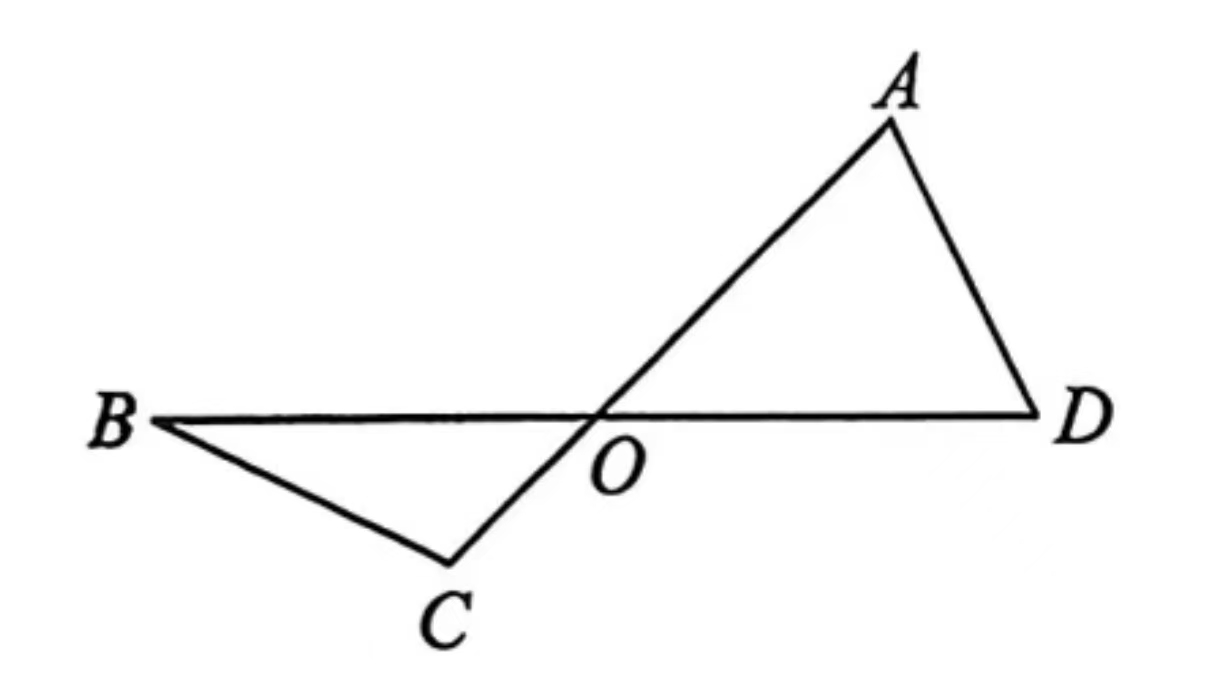
\includegraphics[width=0.3\linewidth]{pi.17.jpg}
        \hspace{1cm} % 可选：图片右侧保留1cm间距（
    \end{figure}

    \newpage
    \item （本小题13分）
    
    一个质点在$x$轴上从原点$O$出发向右运动，每次有$\dfrac{1}{3}$的概率平移$1$一个单位，$\dfrac{2}{3}$的概率平移$2$个单位。设质点运动足够多次时，到达过点$(\ n\ ,\ 0\ )$的概率为$P_n$.
    \begin{enumerate}[label=(\Roman*)]
        \item 求$P_1,P_2$；
        \item 设质点移动$2$次时位于$(\ X\ ,\ 0\ )$，求$X$的分布列与$E(X)$；
        \item 直接用含$n$的式子表示$P_n$.
    \end{enumerate}
    
    \vspace*{\fill}
    \item （本小题15分）
    
    在平面直角坐标系$xOy$中，已知椭圆$T$：$\dfrac{x^2}{4}+y^2=1$，$A$为$T$上顶点，$P$为$T$上异于上、下顶点的动点，$M$为$x$正半轴上的动点.
    \begin{enumerate}[label=(\Roman*)]
        \item 若$P$在第一象限，且$\mid OP \mid =\sqrt{2} $，求$P$的坐标；
        \item 若$\mid MA \mid \ =\ \mid MP \mid$直线$AQ$与$T$交于另一点$C$，且$\overrightarrow{AQ}=2\overrightarrow{AC}\ ,\ \overrightarrow{PQ}=4\overrightarrow{PM}$，求直线$AQ$的方程.
    \end{enumerate}
    \vspace*{\fill}

    \newpage
    \item （本小题15分）从下列两道题中选择一道作答（如果解答全部题目，按分高者计分）

    $a.$已知实数$a \neq 0$，设函数$f(x)=a \ln x+ \sqrt{x+1}\ ,\ x>0$.
    \begin{enumerate}[label=(\Roman*)]
        \item 当$a=-\dfrac{3}{4}$时，求$f(x)$的单调区间；
        \item 若$\forall \ x \in [\ \dfrac{1}{e^2}\ ,\ + \infty\ )$，均有$f(x) \le \dfrac{\sqrt{x}}{2a}$，求$a$的取值范围.
    \end{enumerate}
    $b.$已知函数$f(x)=e^x-e^{-x}-2x$. 
    \begin{enumerate}[label=(\Roman*)]
        \item 讨论$f(x)$的单调性；
        \item 设$g(x)=f(2x)-4bf(x)$，当$x>0$时，$g(x)>0$，求$b$的最大值；
        \item 已知$1.4142<\sqrt{2}<1.4143$，估计$\ln 2$的近似值（精确到$0.001$）.
    \end{enumerate}

    \vspace*{\fill}
    \item 设$A$是由$m \times n$个实数组成的$m$行$n$列的数表，满足：每个数的绝对值不大于$1$，且所有数的和为$0$。设$S(m,n)$为所有这样的数表构成的集合。对于$A \in S(m,n)$，记$r_iA$为$A$的第$i$行各数之和，$C_jA$为$A$的第$j$列各数之和，记$K(A)$为$\mid r_1(A) \mid
    \ ,\ \ldots \ ,\mid r_m(A) \mid\ \ ,\ \mid C_1(A) \mid \ ,\ \ldots \ ,\mid C_m(A) \mid\
    $中的最小值.
    \begin{enumerate}[label=(\Roman*)]
        \item 对如下数表，求$K(A)$;
        
        \begin{tabular}{|c|c|c|}%数表
            \hline
            1 & 1 & -0.8 \\
            \hline
            0.1 & -0.3 & -1 \\
            \hline
        \end{tabular}
        
        \item 设数表$A \in (\ 2\ ,\ 3\ )$，形如以下形式，求$K(A)$的最大值；
        
        \begin{tabular}{|c|c|c|}%数表
            \hline
            1 & 1 & c \\
            \hline
            a & b & -1 \\
            \hline
        \end{tabular}
        
        \item 给定$t \in \mathbb{N^*}$，对于所有$A \in(\ 2\ ,\ 2t+1\ )$，求$K(A)$的最大值.
    \end{enumerate}
    \vspace*{\fill}
    
\end{enumerate}
% =============== 知己知彼pi参考答案 ================
\clearpage %新的一页
\setcounter{enumi}{0}   % 题号从1开始
\phantomsection
\addcontentsline{toc}{section}{参考答案} %加入目录
\setcounter{chapPage}{1} %初始化页数
\fancyfoot[C]{\small 第 \thechapPage 页 /共$2$页} %居中页脚

\begin{center} 
    {\LARGE \textbf{参考答案}}\\[1em]
\end{center}

\sectiontitle{一、选择题（共 $10$ 小题，每小题 $4$ 分，共 $40$ 分）}

    \begin{tasks}[label=(\arabic*), after-item-skip=0.6em](1)
        \task $A$\hfill \makebox[5cm]{（某年\ 华附考试T1）}
        \task $A$\hfill \makebox[5cm]{（21福建质检T1）}
        \task $C$\hfill \makebox[5cm]{（13安徽高考T4）}
        \task $D$\hfill \makebox[5cm]{（24圆创联考T7）}
        \task $A$\hfill \makebox[5cm]{（25武汉二调T8）}
        \task $A$\hfill \makebox[5cm]{（22全国一卷T7） } 
        \task $B$
        \task $C$\hfill \makebox[5cm]{（25雅礼开学T8）}
        \task $B$
        \task $A$\hfill \makebox[5cm]{（24武汉二调T8）}
    \end{tasks}

\sectiontitle{二、填空题（共5小题，每小题5分，共25分）}

    \begin{tasks}[label=(\arabic*), after-item-skip=0.6em,start=11] (1)
        \task $\dfrac{3}{56}$ \hfill \makebox[5cm]{（某年T8联考某题）} 
        \task $6069$ \hfill \makebox[5cm]{（某年\ 广东考试T13）}
        \task $\dfrac{4+\sqrt{7}}{3}$ \hfill \makebox[5cm]{（25上海春考T11）}
        \task $348$\hfill \makebox[5cm]{（某年\ 安徽考试T14）  }
        \task \textcircled{2}  \textcircled{4} \hfill \makebox[5cm]{（24武汉二调T11）}
    \end{tasks}

\sectiontitle{三.解答题（共6小题，共85分）}

    \begin{tasks}[label=(\arabic*), after-item-skip=0.6em,start=16] (1)
        \task 
        (II) \ $\dfrac{\sqrt{3}}{3}$ \hfill\makebox[5cm]{（25佛山一模T15）} \\

        \task
        (II)\ $\sqrt{2}$ \hfill\makebox[5cm]{（25武汉二调T17）}\\[0.6em]

        \task
        (I)\ $P_1=\dfrac{2}{3}\ ,\ P_2=\dfrac{7}{9}$ \\[0.6em]
        (II)\ $EX=\dfrac{33}{16}$\\[0.6EM]
        (III)\ $P_n=\dfrac{1}{4}(-\dfrac{1}{3})^n+\dfrac{3}{4}$\hfill\makebox[5cm]{（25江西八校T18改编）}\\[0.6em]

        \task
        (I)\ $(\ \dfrac{2\sqrt{3}}{3}\ ,\ \dfrac{\sqrt{6}}{3}\ )$ \\[0.6em]
        (II)\ $y=\dfrac{\sqrt{5}}{10}x+1$\hfill\makebox[5cm]{（19 上海春考T21）}\\[0.6em]
        
        \task
        \begin{enumerate}[label=(\alph*)]
            \item 
            (I)\ 单调递减区间为$(\ 0\ ,\ 3\ )$，单调递增区间为$(\ 3\ ,\ +\infty\ )$\\[0.6em]
            (II)\ $(\ 0\ ,\ \dfrac{\sqrt{2}}{4}\ )$\hfill\makebox[5cm]{（19 浙江高考T22）}
            \item 
            (I)\ 函数在$(\ -\infty\ ,\ +\infty\ )$上单调递增\\[0.6em]
            (II)\ $2$\\[0.6em]
            (III)\ $0.693$\hfill\makebox[5cm]{（14 全国II卷 T21）}\\[0.6em]
        \end{enumerate}

        \task
        (I)\ $0.7$\\[0.6em]
        (II)\ $1$\\[0.6em]
        (III)\ $\dfrac{2t+1}{t+2}$\hfill\makebox[5cm]{（12 北京卷 T21）}
    
    \end{tasks}
    
% ================ 知己知彼Sigma ===================
\clearpage %新的一页
\setcounter{enumi}{0}   % 卷II选择题号从1开始
\phantomsection
\addcontentsline{toc}{section}{\texorpdfstring{知己知彼$\Sigma$}{知己知彼Sigma}} % 加入目录
\setcounter{chapPage}{1} %初始化页数
\fancyfoot[C]{\small 高三数学\ 第 \thechapPage 页 (共$5$页)} %居中页脚

\begin{center} 
    {\LARGE \textbf{知己知彼$\Sigma$}}\\[1em]
\end{center}

\sectiontitle{一、选择题共 $10$ 小题，每小题 $4$ 分，共 $40$ 分。在每小题的四个选项中，选出符合题目要求的一项。}

\begin{enumerate}

    \item 集合$A=\{x \mid x^2-2x+3 < 0\}$,集合$B=\{x\mid \dfrac{x+1}{4-x} \ge 0\ ,\ x \in \mathbb{N}^*\}$，则$A\cap B$为
    \begin{tasks}(4)
        \task $\{ 1,2\}$ 
        \task $\{ 0,1,2\}$
        \task $\{ 1,2,3\}$
        \task $\{ 0,1,2,3\}$
    \end{tasks}

    \item 若复数 $z_1=\dfrac{1+2i}{1+i}$ 与 $z_2=\dfrac{3-i}{2+2i}$ ，则$\dfrac{z_2}{z_1}$的共轭复数的虚部为
    \begin{tasks}(4)
        \task $-\dfrac{7}{10}$ 
        \task $-\dfrac{7}{5}$
        \task $\dfrac{7}{10}$
        \task $\dfrac{7}{5}$
    \end{tasks}

    \item 已知命题$p$：关于$x$的不等式$a_1x^2+b_1x+c_1<0$与$a_2x^2+b_2x+c_2<0$的解集相同，命题$q$：$\dfrac{a_1}{a_2}=\dfrac{b_1}{b_2}=\dfrac{c_1}{c_2}$，则$p$是$q$成立的
    \begin{enumerate}[label=(\Alph*)]
        \item 既不充分也不必要条件
        \item 充要条件
        \item 充分不必要条件
        \item 必要不充分条件
    \end{enumerate}

    \item 关于$y=f(x)\ (x\in \mathbb{R})$，$y=f(x-2)$关于$x=2$对称，$x \in (-\infty,0)$时，$f(x)+xf'(x)<0$恒成立。若$a=\dfrac{2}{3}f(\dfrac{2}{3})\ ,\ b=\ln 2f(\ln2)\ ,\ c=\dfrac{3}{4}f(sin^2(\dfrac{\pi}{3}))$，则
    \begin{tasks}(4)
        \task $a<b<C$ 
        \task $a>b>c$
        \task $b>a>c$
        \task $a>c>b$
    \end{tasks}
    
    \item 火箭在发射时,其最大速度 $v$ (单位： $km/s$ )，燃料质量 $M$ (单位： $kg$ )，与除燃料外的火箭质量$N$ (单位： $kg$ )满足：$v=2In(1+\dfrac{M}{N})$。若火箭燃料最大速度为 $16km/s$ ，则下列各数中与$\frac{M}{N}$最接近的是 （参考数据：$\sqrt{2} \approx 1.41$，$\sqrt{3} \approx 1.73$），$\sqrt{5} \approx 2.23$，$\sqrt{7} \approx 2.645$）
    \begin{tasks}(4)
        \task $2000$ 
        \task $3000$
        \task $4000$
        \task $5000$
    \end{tasks}
    \newpage

    \item 已知$x=\dfrac{\pi}{2}$是函数$f(x)= \cos^2 \omega x+ \sin \omega x \cos \omega x=\dfrac{1}{2}$的一个解，且$f(x)$在$(-\dfrac{\pi}{6},\dfrac{\pi}{16})$上单调，则$ \omega =$
    \begin{tasks}(4)
        \task $\dfrac{5}{4}$ 
        \task $\dfrac{7}{4}$
        \task $\dfrac{9}{4}$
        \task $\dfrac{11}{4}$
    \end{tasks}

    \item 在四棱锥$P-ABCD$中，$AB=AD=1$，其他六条棱长均为$2$，则该四棱锥的体积为
    \begin{tasks}(4)
        \task $\dfrac{\sqrt{11}}{6}$ 
        \task $\dfrac{\sqrt{13}}{6}$
        \task $\dfrac{\sqrt{11}}{3}$
        \task $\dfrac{\sqrt{13}}{3}$
    \end{tasks}
    

    \item 在沙漠探索中，每人能带$36$天的生存物资，每人每天能走$30\ km$，且每人都可以在沙漠中将部分生存物资交给其他人然后独自返回。若要求每个人都能顺利返回，且其他人不能再进入沙漠接应，则甲、乙、丙三人合作，甲最远能到达$x_1\ km$。在甲、乙、丙与一个$n$人小队共同合作后，甲最远能到达$x_2\ km$。$x_2-x_1=150\ km$，则$n$为
    \begin{tasks}(4)
        \task $2$
        \task $4$ 
        \task $6$ 
        \task $8$ 
    \end{tasks}

    \item 函数$f(x)=xe^{x+1}-kx+k$有且只有一个负整数$x_0$使$f(x) \le 0$成立，则$k$的取值范围是
    \begin{tasks}(4)
        \task $(\ 0\ ,\ \dfrac{1}{2}\ ]$ 
        \task $(\ 0\ ,\ 1\ )$
        \task $[\ \dfrac{2}{3e}\ ,\ \dfrac{1}{2}\ )$
        \task $(\ \dfrac{2}{3e}\ ,\ \dfrac{1}{2}\ ]$
    \end{tasks}

    \item 函数$f(x)=2\sum_{i=1}^{n} i-n-2n^2 \sin^2 (\dfrac{n \pi}{2})$，且$a_n=f(n)+f(n+1)$,则$\sum_{i=1}^{100} a_i=$
    \begin{tasks}(4)
        \task $0$ 
        \task $100$
        \task $10200$
        \task $-100$
    \end{tasks}
\end{enumerate}

\newpage
\sectiontitle{二、填空题。共5小题，每小题5分，共25分。}
\begin{enumerate}[start=11] % 填空题从11开始编号

    \item$(2x-1)^n=a_nx^n+a_{n-1}x^{n-1}+ \ldots +a_1x+a_0$，则$\dfrac{a_n+a_{n-2}+ \ldots +a_2 +\dfrac{1}{2}a_0}{a_{n-1}+a_{n-3}+ \ldots +a_1 -\dfrac{1}{2}a_0}=$
    \underline{\hspace{2cm}}

    \item 在$\triangle ABC$中，内角$A,B,C$的对边分别为$a,b,c$，则“$a \le \dfrac{\sqrt{2}}{2}(b+c)$”是“$A$是锐角的”\underline{\hspace{2cm}}条件 \ （填“充要”/“既不充分也不必要”/“充分不必要”/“必要不充分”）

    \item 从下列两道题中选择一道作答（如果解答全部题目，按第一个解答计分）
    
    $a$.抛物线$C$的焦点$F$到准线$l$的距离为$2$，$P$是$l$上动点，$A$在$C$上，$\mid AF\mid \ =5$，过$A$作$PF$垂线，垂足为$H$，则$ \mid PH \mid \cdot \mid PF \mid$最小值为
    \underline{\hspace{2cm}}\\
    $b$.双曲线$E=\dfrac{x^2}{a^2}-\dfrac{y^2}{b^2}=1\ (a>0,\ b>0)$，过原点做一条倾斜角为$\dfrac{\pi}{3}$的直线，分别与双曲线$E$左右两支交于$P,Q$点，若$\triangle PQF$为锐角三角形，则离心率$e$的取值范围是\underline{\hspace{2cm}}

    \item 四边形$ABCD$，$\overrightarrow{AB}=2\overrightarrow{DC},\ AB=4,\ BC=AD=2\ ,E,F,G$在$AB,BD,AC$上，$\dfrac{AE}{AB}=\dfrac{BF}{BD}=\dfrac{AG}{AC}=\lambda$，设$CE \ \cap \ GF=I $,则IF最小值为 
    \underline{\hspace{2cm}}；
    当$\overrightarrow{AE} \cdot \overrightarrow{DF}<0$时，$\lambda$的取值范围是\underline{\hspace{2cm}}

    \item 设函数$f(x) =
        \begin{cases}
        a(x+\dfrac{\pi}{2}), & x <\dfrac{\pi}{2} \\
        \cos x, & \dfrac{\pi}{2}<x < \pi \\
        e^{-x+\pi}+4a, &x>\pi
        \end{cases}$
        ，则下列说法正确的是
        \underline{\hspace{2cm}}\\[1em]
    \textcircled{1}  若$f(x)$有最小值，则$a \in [\ \dfrac{1}{\pi},0\ ]$；\\
    \textcircled {2} 若当$a>0$时，$f(x)=t$无实根，则$t \in [\ a\pi,4a\ ]\cup[\ 4a+1,+\infty\ )$；\\
    \textcircled {3} $a \le -\dfrac{1}{2}$时，$f(x^2+2)>f(\ \mid x \mid +4)$的解集为$(\ -2,2\ )$；\\
    \textcircled {4} 当$a \ge 1$时，存在$x_1<x_2$，$-1<f(x_1)=f(x_2)<0$，则$x_1+x_2>0$ 
    
\end{enumerate}


\newpage
\sectiontitle{三.解答题。共6小题，共85分。解答应写出文字说明，演算步骤或证明过程。}

\begin{enumerate}[start=16] %大题从16开始编号

    \item （本小题13分）

    某城市运动公园如图，锐角$\triangle ABE$为球类区，四边形$BCDE$为文艺区，已知$BC=3\ ,\ BD=3\sqrt{3}\ ,\ DE=6\ ,\ CE=3\sqrt{7}\ ,\ \angle BCD=120^\circ $.
    \begin{enumerate}[label=(\Roman*)]
        \item   求$BE$的长度；
        \item 若$\angle BAE=60^\circ$，求球类区面积的取值范围.
    \end{enumerate}
    
    \begin{figure}[htbp]
        \hfill %表示“填充剩余空间”，实现靠右+自定义间距
        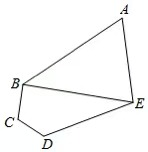
\includegraphics[width=0.22\linewidth]{Sigma.16.jpg}
        \hspace{1cm} % 可选：图片右侧保留1cm间距（
    \end{figure}

    \item （本小题14分）
    
    如图，在三棱柱$ABC-A_1B_1C_1$中，$\angle ACB=90 ^\circ$，$D$为$AC$中点，且$A_1D \perp $面$ABC$.
    \begin{enumerate}[label=(\Roman*)]
        \item 证明：面$A_1BC \perp$面$AA_1CC_1$；
        \item 证明：$B_1C \parallel $面$A_1BD$；
        \item 若$A_1B \perp A_1C\ ,\ AC=BC=2$，求三棱柱$ABC-A_1B_1C_1$的表面积.
    \end{enumerate}
    
    \begin{figure}[htbp]
        \hfill %表示“填充剩余空间”，实现靠右+自定义间距
        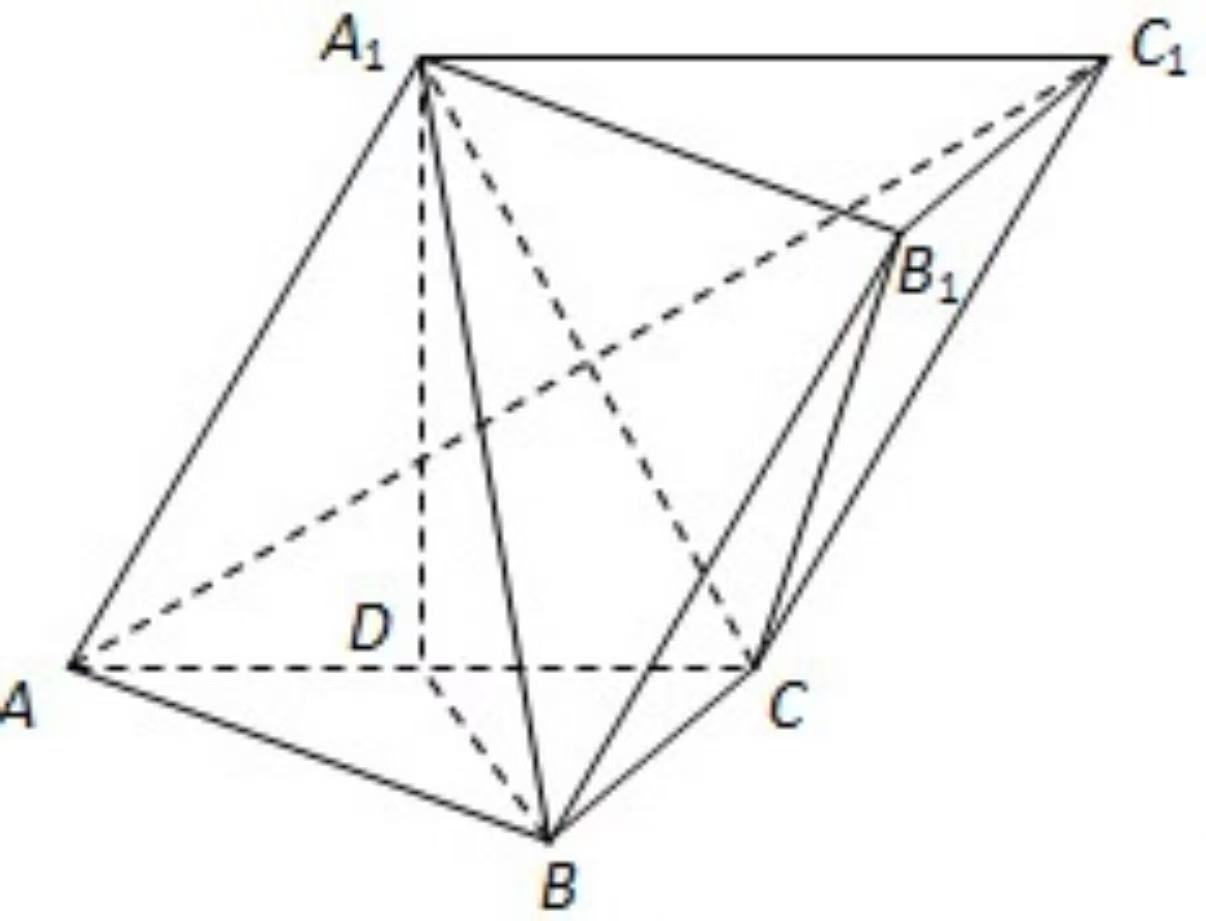
\includegraphics[width=0.3\linewidth]{Sigma.17.jpg}
        \hspace{1cm} % 可选：图片右侧保留1cm间距（
    \end{figure}


    \newpage
    \item （本小题13分）
    
    甲、乙进行羽毛球比赛。比赛规定：一回合赢球的一档作为下一回合发球方，若甲发球，则本回合甲赢的概率为$\dfrac{3}{4}$；若乙发球，则本回合甲赢的概率为$\dfrac{1}{4}$。每回合结果相互独立，第一回合由甲发球.
    \begin{enumerate}[label=(\Roman*)]
        \item 求第三回合乙发球的概率；
        \item 设前三个回合甲发球次数为$X$，求$X$的分布列和期望；
        \item 设第$n$个回合甲发球概率为$P_n$，直接写出$P_N$表达式.
    \end{enumerate}
    
    \item （本小题15分）
    
    已知椭圆$C$：$\dfrac{x^2}{a^2}+\dfrac{y^2}{b^2}=1\ (a>b>0)$的离心率为$\dfrac{1}{2}$，左顶点为$(-2\sqrt{2},0)$.
    \begin{enumerate}[label=(\Roman*)]
        \item 求$C$的方程；
        \item 设直线$l:y=kx+m\ (m \neq 0)$与$E$交于$A,B$点，过$B$作$y=3 \sqrt{3}$的垂线，垂足为$D$，当$AD$与$y$轴交于定点时，求$m$.
    \end{enumerate}

    \item （本小题15分）

    设函数$f(x)=(\dfrac{a}{x}-1) \ln x+1 \ (a \in \mathbb{R})$
    \begin{enumerate}[label=(\Roman*)]
        \item 若$f(x)$在 $x=2$处的切线于$y=-\dfrac{\ln 2}{2}x$平行；
         \begin{enumerate}[label=(\roman*)]
         \item 求$a$;
         \item 证明：$f(x)$有且只有两个零点；
         \end{enumerate}
        \item 设函数$g(x)=e^x-x(f(x)+\ln x-1)$，若$g(x)$在区间$(\ 0\ ,\  e^{-a}\ )$上存在极值，求证：$a^{-1}+e^{-a}>a+1$.
    \end{enumerate}
    
\end{enumerate}

% ============== 知己知彼Sigma参考答案 ================
\clearpage %新的一页
\setcounter{enumi}{0}   % 题号从1开始
\phantomsection
\addcontentsline{toc}{section}{参考答案} %加入目录
\setcounter{chapPage}{1} %初始化页数
\fancyfoot[C]{\small 第 \thechapPage 页 /共$1$页} %居中页脚

\begin{center} 
    {\LARGE \textbf{参考答案}}\\[1em]
\end{center}

\sectiontitle{一、选择题（共 $10$ 小题，每小题 $4$ 分，共 $40$ 分）}

    \begin{tasks}[label=(\arabic*), after-item-skip=0.6em,start=1] (5)
        \task $A$ 
        \task $A$
        \task $A$
        \task $B$        
        \task $B$
        \task $B$        
        \task $C$
        \task $C$        
        \task $D$
        \task $D$
    \end{tasks}

\sectiontitle{二、填空题（共5小题，每小题5分，共25分）}

    \begin{tasks}[label=(\arabic*), after-item-skip=0.6em,start=11] (2)
        \task $-1$ 
        \task 既不充分也不必要
        \task $a.\ 6$\ \ \ \ $b.\ (\ \sqrt{3}+1,\sqrt{3}+\sqrt{7}\ )$
        \task $\dfrac{7}{4}$，$(\ 0,\dfrac{7-\sqrt{33}}{4}\ )$  
        \task \textcircled{2} \textcircled{3} \textcircled{4}
        \end{tasks}

\sectiontitle{三.解答题（共6小题，共85分）}

    \begin{tasks}[label=(\arabic*), after-item-skip=0.6em,start=16] (1)
        \task 
        (I) \ $3 \sqrt{7}$\\[0.6em]
        (II) \ $(\ \dfrac{21 \sqrt{3}}{2},\dfrac{63 \sqrt{3}}{4}\ )$ \\

        \task
        (III)\ $2 \sqrt{3}$\\

        \task
        (I)\ $\dfrac{3}{8}$ \\[0.6em]
        (II)\ $EX=\dfrac{33}{16}$\\[0.6EM]
        (III)\ $P_n=(\dfrac{1}{2})^n+\dfrac{1}{2}$\\

        \task
        (I)\ $\dfrac{x^2}{16}+\dfrac{y^2}{8}= 1$ \\[0.6em]
        (II)\ $m=\dfrac{4 \sqrt{2}}{3}$\\
        
        \task
        (I)(i)\ $a=2$\\[0.6em]
    
    \end{tasks}

% ================ 知己知彼i ===================
\clearpage %新的一页
\setcounter{enumi}{0}   % 卷II选择题号从1开始
\phantomsection
\addcontentsline{toc}{section}{\texorpdfstring{知己知彼$i$}{知己知彼i}} % 加入目录
\setcounter{chapPage}{1} %初始化页数
\fancyfoot[C]{\small 高三数学\ 第 \thechapPage 页 (共$6$页)} %居中页脚

\begin{center} 
    {\LARGE \textbf{知己知彼$i$}}\\[1em]
\end{center}

\sectiontitle{一、选择题共 $10$ 小题，每小题 $4$ 分，共 $40$ 分。在每小题的四个选项中，选出符合题目要求的一项。}

\begin{enumerate}

    \item 阅读下段文字：“已知$\sqrt{2}$为无理数，若$(\sqrt{2})^{\sqrt{2}}$为有理数，则存在无理数$a=b=\sqrt{2}$，使得$a^b$为有理数；若$(\sqrt{2})^{\sqrt{2}}$为无理数，则取无理数$a=(\sqrt{2})^{\sqrt{2}}\ ,\ b=\sqrt{2}$，此时$a^b=((\sqrt{2})^{\sqrt{2}})^{\sqrt{2}}=(\sqrt{2})^{\sqrt{2}\sqrt{2}}=(\sqrt{2})^2=2$为有理数。”依据这段文字可以证明的结论是
    \begin{tasks}(2)
        \task $(\sqrt{2})^{\sqrt{2}}$是有理数 
        \task $(\sqrt{2})^{\sqrt{2}}$是无理数
        \task 存在无理数$a\ ,\ b$，使得$a^b$为有理数
        \task 对任意无理数$a\ ,\ b$，都有$a^b$为无理数
    \end{tasks}

    \item 设复数 $z_1$，$z_2$满足$z_2\neq0$，且$\mid z_1 \cdot z_2 \mid=2 \mid z_2 \mid$，则$z_1$可以是
    \begin{tasks}(4)
        \task $-1-i$ 
        \task $2+2i$
        \task $-1+\sqrt{3}i$
        \task $4i$
    \end{tasks}

    \item 函数$f(x)= \dfrac{2\tan x}{1-\tan ^2 x}$的最小正周期是
    \begin{tasks}(4)
        \task $\dfrac{\pi}{4}$ 
        \task $\dfrac{\pi}{2}$
        \task $\pi$
        \task $2\pi$
    \end{tasks}

    \item 已知直线$m$与平面$\alpha$所成的角为$\dfrac{\pi}{4}$，若直线$n \subset \alpha$，直线$m \subset \beta$，设$m$与$n$的夹角为$\theta_1$，$\alpha$与$\beta$的夹角为$\theta_2$，则
    \begin{tasks}(2)
        \task $\theta_1 \ge \dfrac{\pi}{4}\ ,\ \theta_2 \ge \dfrac{\pi}{4} $
        \task $\theta_1 \ge \dfrac{\pi}{4}\ ,\ \theta_2 \le \dfrac{\pi}{4} $
        \task $\theta_1 \le \dfrac{\pi}{4}\ ,\ \theta_2 \ge \dfrac{\pi}{4} $
        \task $\theta_1 \le \dfrac{\pi}{4}\ ,\ \theta_2 \le \dfrac{\pi}{4} $
    \end{tasks}
    
    \item 已知函数$f(x)=A \sin (\omega x+\phi)$的部分图像如图所示，其中$A>0\ ,\ \omega >0\ ,\ -\dfrac{\pi}{2}<\phi<0$。在已知$\dfrac{x_2}{x_1}$的条件下，下列选项中可以确定其值的量为
    \begin{tasks}(4)
        \task $\omega$ 
        \task $\phi$
        \task $\dfrac{\phi}{\omega}$
        \task $A \sin \phi$
    \end{tasks}
    
    \begin{figure}[htbp]
        \hfill %表示“填充剩余空间”，实现靠右+自定义间距
        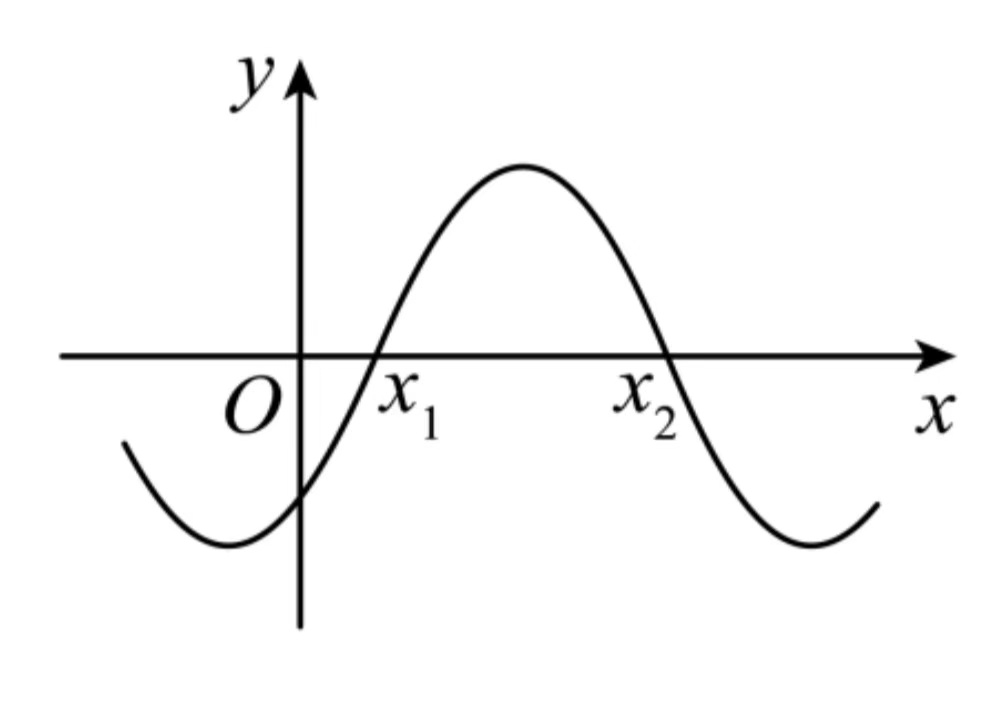
\includegraphics[width=0.22\linewidth]{i.5.jpg}
        \hspace{1cm} % 可选：图片右侧保留1cm间距（
    \end{figure}
    \newpage

    \item 已知连续型随机变量$\xi$服从正态分布$N(\dfrac{1}{2}\ ,\ \dfrac{1}{4})$,记函数$f(x)=P(\xi \le x)$，则$f(x)$ 的图像 
    \begin{tasks}(2)
        \task 关于直线$x=\dfrac{1}{2}$对称 
        \task 关于直线$x=\dfrac{1}{4}$对称
        \task 关于点$(\dfrac{1}{2},\dfrac{1}{2})$成中心对称
        \task 关于点$(\dfrac{1}{4},\dfrac{1}{4})$成中心对称
    \end{tasks}

    \item 已知$S_n$是等比数列的前$n$项和，则“$a_2,a_8,a_5$依次成等差数列”是“$S_3,S_9,S_6$依次成等差数列”的
    \begin{enumerate}[label=(\Alph*)]
        \item 充分不必要条件
        \item 必要不充分条件
        \item 充要条件
        \item 既不充分也不必要条件
    \end{enumerate}
    

    \item 已知函数$f(x)=2 \cos (\omega x+ \dfrac{\pi}{6})\ ,\ x \in [-\pi,0]$，若$f(x)$恰有$3$个极值点，则正数$\omega$的取值范围为
    \begin{tasks}(4)
        \task $[\ \dfrac{8}{3}\ ,\ \dfrac{11}{3}\ )$ 
        \task $(\ \dfrac{8}{3}\ ,\ \dfrac{11}{3}\ ]$
        \task $[\ \dfrac{13}{6}\ ,\ \dfrac{19}{6}\ )$
        \task $(\ \dfrac{13}{6}\ ,\ \dfrac{19}{6}\ ]$
    \end{tasks}

    \item 设$a \in \mathbb{R}$，函数$f(x) =
        \begin{cases}
        \sin \ (2 \pi x-2 \pi a), & x <a \\
        \mid x-a-1 \mid-3a+6, & x \ge a
        \end{cases}$
        ，若在区间$(0,+\infty)$内恰有6个零点，则$a$的取值范围为
    \begin{tasks}(2)
        \task $(\ 2\ ,\ \dfrac{7}{2}\ ]$ 
        \task $(\ 2\ ,\ 3\ ]$
        \task $[\ 2\ ,\ \dfrac{7}{3}\ )\ \cup\ (\ \dfrac{5}{2}\ ,\ \dfrac{7}{2}\ ]$
        \task $[\ 2\ ,\ \dfrac{7}{3}\ )\ \cup\ (\ \dfrac{5}{2}\ ,\ 3\ ]$
    \end{tasks}

    \item 已知函数$f(x)$，$g(x)$的定义域均为$\mathbb{R}$,且函数$f(x)$的图像关于点$(2,0)$对称，设集合$A=\{\ a \mid \forall \ x\in \mathbb{R} \ ,\ f(x)+g(a)>0\}$，$B=\{\ a \mid \exists \ x\in \mathbb{R} \ ,\ f(x)+g(a)>0\}$，$C=\{\ a \mid g(a) \ge f(1)\ \}$，则
    \begin{tasks}(4)
        \task $A \cap C=A$ 
        \task $A \cap C=C$
        \task $B \cap C=B$
        \task $B \cap C=C$
    \end{tasks}
\end{enumerate}

\newpage
\sectiontitle{二、填空题。共5小题，每小题5分，共25分。}
\begin{enumerate}[start=11] % 填空题从11开始编号

    \item 直线$l_1:\ y=2x$和$l_2:\ y=kx+1$与$x$轴围成的三角形是等腰三角形，写出满足条件的$k$的两个可能取值：
    \underline{\hspace{2cm}}和\underline{\hspace{2cm}}

    \item 已知等差数列$\{a_n\}$的公差$d \neq 0$，若$a_2,\ a_5,\ a_9$构成等比数列，则$\dfrac{a_2}{a_1}=$ 
    \underline{\hspace{2cm}}

    \item 已知函数$f(x)=e^x-e^{1-x}-ax$有两个极值点$x_1$和$x_2$，若$f(x_1)+f(x_2)=-4$，则实数$a=$
    \underline{\hspace{2cm}}

    \item 所有顶点都在两个平行平面内的多面体叫拟柱体。在这两个平行平面内的面叫做拟柱体的底面，其余各面叫做拟柱体的侧面，两底面之间的垂直距离叫做拟柱体的高，现有一拟柱体，上下底面均为正六边形，且下底面边长为$4$，上地面各顶点在下底面的射影点为下底面各边的中点，高为$2$，则该拟柱体的体积为
    \underline{\hspace{2cm}}
    
    \item 已知曲线$C$的方程为$x^2+y^2+axy=1$，则下列说法正确的是\underline{\hspace{2cm}}\\[1em]
    \textcircled{1}  无论$a$取何值，曲线$C$都关于原点中心对称；\\
    \textcircled {2} 存在唯一的实数$a$使得曲线$C$表示两条直线；\\
    \textcircled {3} 当$a=1$时，曲线$C$上任意两点间距离的最大值为$2\sqrt{2}$；\\
    \textcircled {4} 当$a>2$时，曲线$C$是双曲线
    
\end{enumerate}


\newpage
\sectiontitle{三.解答题。共6小题，共85分。解答应写出文字说明，演算步骤或证明过程。}

\begin{enumerate}[start=16] %大题从16开始编号

    \item （本小题13分）

    在四棱锥$P-ABCD$中，底面$ABCD$为直角梯形，$AD\parallel BC\ ,\ AB \perp AD\ ,\ PA \perp$平面$ABCD\ .\ AP=AD=2AB=4BC$.
    \begin{enumerate}[label=(\Roman*)]
        \item 求证：平面$PAC \perp$平面$PBD$；
        \item $AM \perp $平面$PCD$于$M$，求二面角$M-AD-P$的余弦值.
    \end{enumerate}
    
    \begin{figure}[htbp]
        \hfill %表示“填充剩余空间”，实现靠右+自定义间距
        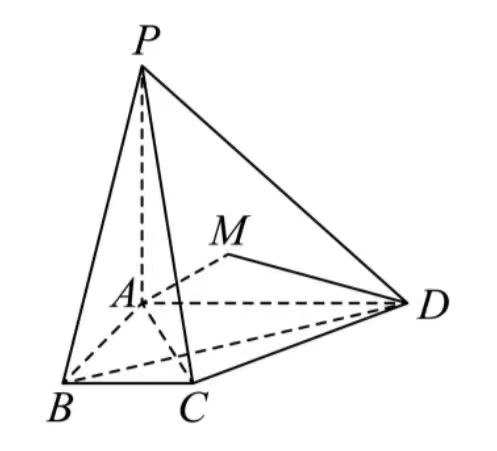
\includegraphics[width=0.22\linewidth]{i.16.jpg}
        \hspace{1cm} % 可选：图片右侧保留1cm间距（
    \end{figure}

    \item （本小题14分）
    
    在$\triangle ABC$中，$AB=2$，$D$为$AB$中点.
    \begin{enumerate}[label=(\Roman*)]
        \item 若$BC=\sqrt{2}$，求$AC$的长；
        \item 若$\angle BAC=2 \angle BCD$，求$AC$的长；
    \end{enumerate}

    \newpage
    \item （本小题13分）
    
    PageRank 算法是 Google搜索引擎用来衡量网页重要性的一种经典算法，其核心思想是通过分析网页之间的链接关系，评估每个网页的相对重要性．假设一个小型的互联网由A，B，C，D四个网页组成，它们之间按图中的箭头方向等可能地单向链接，假设某用户从网页A开始浏览（记沩第1 次停留）.
    \begin{enumerate}[label=(\Roman*)]
        \item 求该用户第$3$次停留在网页D上的概率；
        \item 某广告公司准备在网页B，C中选择一个投放广告，以用户前$4$次在该网页上停留的平均次数作为决策依据.试问该公司应该选择哪个网页？请说明理由
    \end{enumerate}

    \begin{figure}[htbp]
        \hfill %表示“填充剩余空间”，实现靠右+自定义间距
        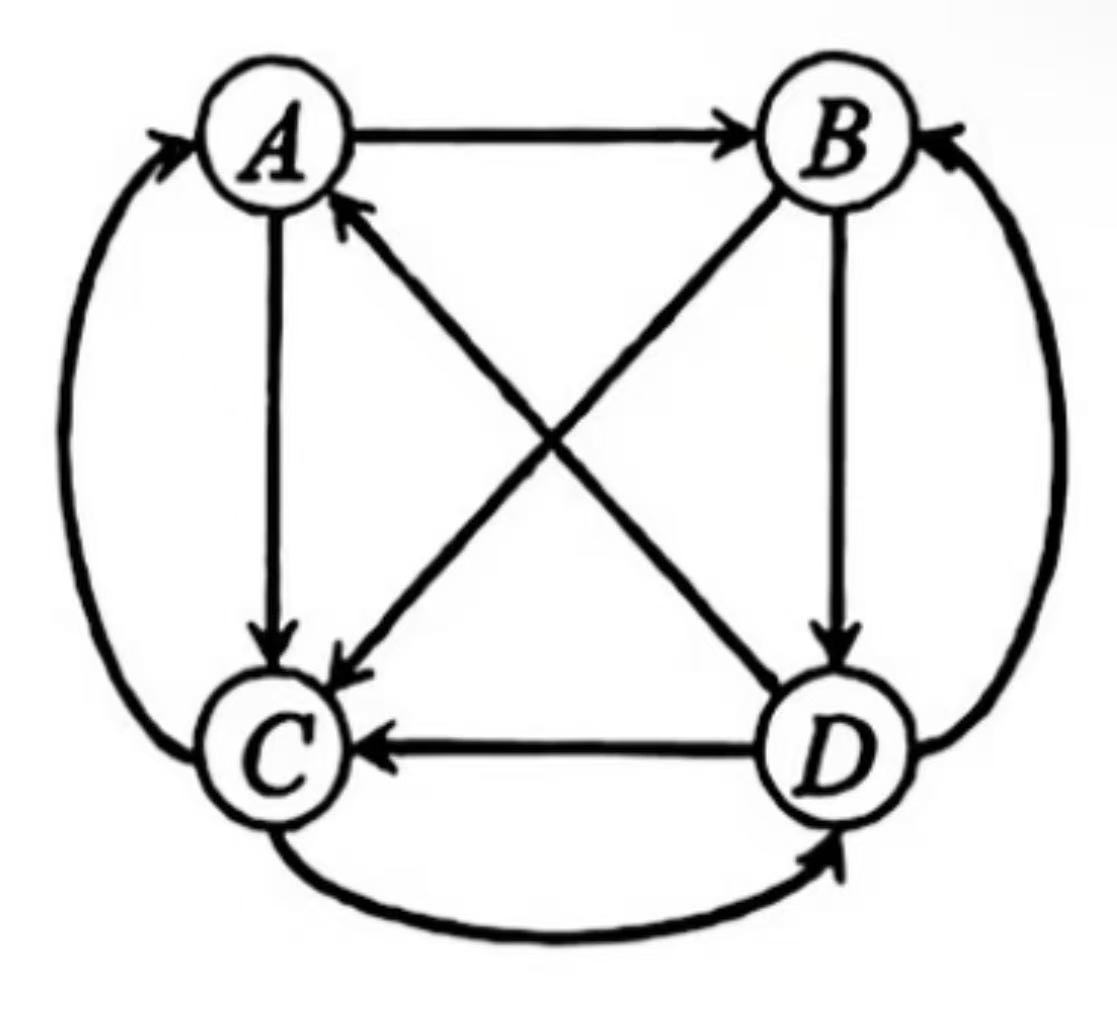
\includegraphics[width=0.22\linewidth]{i.18.jpg}
        \hspace{1cm} % 可选：图片右侧保留1cm间距（
    \end{figure}
    
    \item （本小题15分）
    
    已知$P,Q\ (\ 2 \sqrt{2},2\ )$在椭圆$E$：$\dfrac{x^2}{a^2}+\dfrac{y^2}{b^2}=1\ (a>b>0)$上，$F_2$为右焦点，$PF_2 \perp x$轴且$\mid PF_2 \mid =2 $.
    \begin{enumerate}[label=(\Roman*)]
        \item 求$E$的标准方程；
        \item 设点$P(-2\sqrt{2}\ ,\ 3)\ ,\ Q(2\sqrt{2}\ ,\ 3)$，$R$为$C$上一点且在$x$轴上方，直线$PQ\ ,\ QR$分别交$x$轴于$M$，$N$两点若$\triangle PQR$的面积比$\triangle MNR$的面积大$3\sqrt{2}$，求点$R$的坐标.
    \end{enumerate}
    
    \newpage
    \item （本小题15分）

    已知函数$f(x)=\ln (x+1)+\dfrac{ax}{x+1}\ (a \in \mathbb{R}) $
    \begin{enumerate}[label=(\Roman*)]
        \item 讨论$f(x)$的单调性；
        \item 若$f(x)$在区间$(\ -1\ ,\  0\ )$上恰有一个零点，求$a$的取值范围；
        \item 当$a>0$时，解方程$f^{'}(x)-f(x)=\dfrac{\sqrt{5}-1}{2}-\ln \dfrac{\sqrt{5}-1}{2}$.
    \end{enumerate}

    \vspace*{\fill}
    \item 已知$r$是给定的正整数，设$G$是以满足下列条件\textcircled{1} \textcircled{2} \textcircled{3}的函数$f(x)$为元素构成的集合:\\
    \textcircled{1}\ ：定义域为$[\ 0\ ,\ r\ ]$\ ;\\
    \textcircled{2}\ ：$f(0)=0$\ ;\\
    \textcircled{3}\ ：$f(x)=f(k)+a_k(x-k)\ ,\ k<x \le k+1$，其中$a_k \in \{-1,2\}$，$k \in\{0,1,2,\cdots,r-1\}$\ .\\
    对给定的整数$m$，$n$（其中$0 \le n \le r$），记$A_{n,m}=\{f(x)\in G\mid f(n)=m\}$.
    \begin{enumerate}[label=(\Roman*)]
        \item 当$r=2$时，直接写出集合$A_{2,-2}$和$A_{2,1}$（无需说明推导过程）；
        \item 若$0 \le i<j \le r$且$j-i$不是$3$的倍数，证明：$A_{i,m} \cap A_{j,m}= \emptyset$；
        \item 从集合$G$中随机取出一个函数$g(x)$，证明：对任意$0 <n \le r-3$，随机事件“$g(x) \in A_{n,m} \cap A_{n+3,m}$”发生的概率都不超过$\dfrac{3}{16}$.
    \end{enumerate}
    \vspace*{\fill}
    
\end{enumerate}

% ============== 知己知彼i参考答案 ===============
\clearpage %新的一页
\setcounter{enumi}{0}   % 题号从1开始
\phantomsection
\addcontentsline{toc}{section}{参考答案} %加入目录
\setcounter{chapPage}{1} %初始化页数
\fancyfoot[C]{\small 第 \thechapPage 页 /共$1$页} %居中页脚

\begin{center} 
    {\LARGE \textbf{参考答案}}\\[1em]
\end{center}

\sectiontitle{一、选择题（共 $10$ 小题，每小题 $4$ 分，共 $40$ 分）}

    \begin{tasks}[label=(\arabic*), after-item-skip=0.6em,start=1] (5)
        \task $C$ 
        \task $C$
        \task $C$
        \task $A$        
        \task $B$
        \task $C$        
        \task $B$
        \task $D$        
        \task $D$
        \task $A$
    \end{tasks}

\sectiontitle{二、填空题（共5小题，每小题5分，共25分）}

    \begin{tasks}[label=(\arabic*), after-item-skip=0.6em,start=11] (2)
        \task $-2$，$\dfrac{\sqrt{5}-1}{2}$（答案不唯一） 
        \task $\dfrac{9}{8}$
        \task $4$
        \task $44 \sqrt{3}$        
        \task \textcircled{1} \textcircled{3} \textcircled{4}
    \end{tasks}

\sectiontitle{三.解答题（共6小题，共85分）}

    \begin{tasks}[label=(\arabic*), after-item-skip=0.6em,start=16] (1)
        \task 
        (II) \ $\dfrac{2 \sqrt{13}}{13}$ \\

        \task
        (I)\ $2$\\[0.6em]
        (II)\ $\dfrac{-1+\sqrt{17}}{2}$ \\

        \task
        (I)\ $\dfrac{1}{2}$ \\[0.6em]
        (II)\ 应该选择$C$网页。原因：求出$E(B)$与$E(C)$，$E(C)>E(B)$\\[0.6em]

        \task
        (I)\ $\dfrac{x^2}{8}+\dfrac{y^2}{6}= 1$ \\[0.6em]
        (II)\ $(\pm\dfrac{2\sqrt{15}}{3}\ ,\ 1\ )$\\
        
        \task
        (I)\ 当$a \ge 0$时，$f(x)$在定义域内单调递增；\\[0.6em]
        当$a<0$时，$f(x)$在$(-1,-1-a)$上单调递减；在$(-1-a,+ \infty)$上单调递增\\[0.6em]
        (II)\ $(-1,0)$\\[0.6em]
        (III)\ $x=\dfrac{\sqrt{5}-1}{2}$

        \task
        (I) $A_{2,-2}=\{y=-x,\ 0\le x\le 2\}$；\\
        $A_{2,1}=\big\{y= \begin{cases}
        -x, & 0\le x\le 1 \\
        2x-3, & 1<x\le 2
        \end{cases},\ y= \begin{cases}
        2x, & 0\le x\le 1 \\
        -x+3, & 1<x\le 2
        \end{cases}\big\}$；\\[0.6em]
    
    \end{tasks}
    
%================= 知己知彼Omega ===================
\newpage
\phantomsection
\addcontentsline{toc}{section}{\texorpdfstring{知己知彼$\Omega$}{知己知彼Omega}} % 加入目录
\setcounter{chapPage}{1} %初始化页数
\fancyfoot[C]{\small 高三数学\ 第 \thechapPage 页 (共$8$页)} %居中页脚

\begin{center}%标题
    {\LARGE \textbf{知己知彼$\Omega$}}\\[1em]
\end{center}

\sectiontitle{一、选择题共 $10$ 小题，每小题 $4$ 分，共 $40$ 分。在每小题的四个选项中，选出符合题目要求的一项。}

\begin{enumerate}

    \item 集合$A=\{(x,y) \mid y \ge x^2\}$,集合$B=\{(x,y)\mid y \le 2x\}$，设$A \cap B$中所有元素构成图形的面积为$S$。你也许不会求解$S$，但是你可以利用$y=x^2$在$x=1$和$x=2$处的切线来估计$S$的值,则下列数值中大于$S$且最接近$S$的是
    \begin{tasks}(4)
        \task $\dfrac{5}{4}$ 
        \task $\dfrac{7}{4}$
        \task $\dfrac{9}{4}$
        \task $\dfrac{11}{4}$
    \end{tasks}

    \item 若复数 $z_1$ 与 $z_2$ 满足 $\dfrac{z_2}{z_1}=i^a $， $a \in \mathbb{N}$， 则在复平面中, $z_1$ 与$z_2$ 的夹角可能是
    \begin{tasks}(4)
        \task $\dfrac{\pi}{2}$ 
        \task $\dfrac{\pi}{3}$
        \task $\dfrac{\pi}{4}$
        \task $\dfrac{\pi}{6}$
    \end{tasks}

    \item 已知平面向量 $\boldsymbol{a}$，$\boldsymbol{b}$，满足$|\ \boldsymbol{a} \  |=2$，$ \boldsymbol{a} \cdot \boldsymbol{b} = |\ k \boldsymbol{b}\ |$，则“$|\ \boldsymbol{b} - \boldsymbol{a} \ |$的最小值是$\sqrt3$”是“$k=\dfrac{1}{2}$”的
    \begin{enumerate}[label=(\Alph*)]
        \item 充要条件
        \item 充分不必要条件
        \item 必要不充分条件
        \item 既不充分也不必要条件
    \end{enumerate}

    \item 设直线$l_1: x+y-2=0$与$x$轴和$y$轴交点分别是$A$ 、 $B$，直线$l_2:kx-y+1=0$ 与直线 $l_3:x+ky-1=0$交于$C$, 则  $\overrightarrow{AC} \cdot \overrightarrow{BC} $的取值范围是
    \begin{tasks}(4)
        \task $(0,2]$ 
        \task $[0,2)$
        \task $(-2,0]$
        \task $[-2,0)$
    \end{tasks}
    \newpage
    
    \item 对数在物理学中有着广泛的应用。火箭在发射时,其最大速度 $v$ (单位： $km/s$ )，燃料质量 $M$ (单位： $kg$ )，与除燃料外的火箭质量$N$ (单位： $kg$ )满足：$v=2In(1+\dfrac{M}{N})$。若火箭燃料提供的最大速度约为 $16km/s$ ，则下列数值中与火箭发射时$\frac{M}{N}$最接近的是 （参考数据：$e \approx 2.7$，$\sqrt{30} \approx 5.4$）
    \begin{tasks}(4)
        \task $2000$ 
        \task $2500$
        \task $3000$
        \task $3500$
    \end{tasks}

    \item 设函数$f(x)= \sin (\omega x+ \phi)\  (\omega  > 0,\ 0 < \phi < \frac{\pi}{2})$，$f (\dfrac{5}{16}) = 0$，$f(x)$在$x= －\dfrac{1}{4}$处取得最小值，且$[\ \dfrac{1}{2}\ ,\ \dfrac{3}{4}\ ]$是$f(x)$的一个增区间，则$ \omega =$
    \begin{tasks}(4)
        \task $\dfrac{8\pi}{9}$ 
        \task $\dfrac{8\pi}{3}$
        \task $\dfrac{40\pi}{9}$
        \task 以上都不对
    \end{tasks}

    \item 一个不透明盒子中有 $3$ 个相同的球，其中有 $2$ 个橙球，$1$ 个白球。甲和乙两个人会从中抽 $2$ 个球并记录抽出球的颜色，其中甲每抽完一个球就放回去，乙抽完球不放回。
    设甲抽出的橙球数量为$X$ ，$X$ 的期望为 $E(X)$，方差为$D(X)$；乙抽出的橙球量数为$Y$ ，$Y$的期望为$E(Y)$，方差为$D(Y)$。则下列说法正确的是  
    \begin{enumerate}[label=(\Alph*)]
        \item $E(X)>E(Y)$，$D(X)=D(Y)$
        \item $E(X)=E(Y)$，$D(X)<D(Y)$
        \item $E(X)=E(Y)$，$D(X)=D(Y)$
        \item $E(X)=E(Y)$，$D(X)>D(Y)$
    \end{enumerate}
    
\newpage
    \item 已知椭圆$E1$：$\dfrac{x^2}{a^2}+\dfrac{y^2}{b^2}=1$与双曲线$E2$：$\dfrac{y^2}{a^2}-\dfrac{x^2}{b^2}=1\ (a \neq b \neq 0)$，$O$为坐标轴原点，则下列说法正确的个数是\\
        \textcircled{1} $E1$ 与 $E2$ 可能有$0$、$2$或$4$个交点\\
        \textcircled{2} "$E1$ 与 $E2$无交点”的充要条件是“$a>b>0$”\\
        \textcircled{3} 若$E1$ 与 $E2$有四个交点$A,B,C,D$分别位于第一、二、三、四象限，$\triangle ABO$为等边三角形，则$E2$ 与 $E1$离心率之比为$\sqrt6$
    \begin{tasks}(4)
        \task $0$ 个
        \task $1$ 个
        \task $2$ 个
        \task $3$ 个
    \end{tasks}

    \item  已知三棱锥$P-ABC$ 中，$Q$ 为 $PC$ 中点，$D$ 为$AC$ 中点，$PB\perp AB$ ，$QB=2$ ，$PA=2\sqrt2$， $BC=\sqrt3$，$cos \angle  QDB=－\dfrac{\sqrt2}{4}$，$\triangle ABC$的周长为$3+\sqrt3$，则 $PC$与面$ABC$夹角余弦值为
    \begin{tasks}(4)
        \task $\dfrac{\sqrt2}{2}$ 
        \task $\dfrac{\sqrt 3}{2}$
        \task $\dfrac{\sqrt6}{3}$
        \task 以上都不对
    \end{tasks}

    \item 数学课上，老师给出了曲线$E$的表达式：$f(\sin 2x)=\sin x$，对于$f(x)$是否为一个函数，同学们产生了质疑，则下列说法正确的是
    \begin{enumerate}[label=(\Alph*)]
        \item 取$x=\dfrac{\pi}{4}$和$x=\dfrac{3\pi}{4}$能够证明$f(x)$不是函数
        \item 若$\sin x_1=\sin x_2$，$\sin (2x_1)\neq \sin (2x_2)$有解，则不能证明$f(x)$不是函数
        \item 设$y=\sin x$，$t=\sin (2x)$，则曲线$E$满足$t^2+(2y^2-1)^2=1$
        \item 设$y=\sin x$，$t=\sin (2x)$，则曲线$E$满足$y^2+(2t^2-1)^2=1$
    \end{enumerate}
\end{enumerate}

\newpage
\sectiontitle{二、填空题。共5小题，每小题5分，共25分。}
\begin{enumerate}[start=11] % 填空题从11开始编号

    \item$(x-2y+3)^5$中$x^2 y$的系数为\underline{\hspace{2cm}}

    \item 一个$4$层阶梯金字塔，其每一层都可视为相似的正四棱台。正四棱台顶边与底边长度之比为$4:5$，上下相邻两层底边长度之比为$3:5$，侧面与底面夹角正切值为$\sqrt3$，底面边长为$a$，则该金字塔的高度为
    \underline{\hspace{2cm}}
    （用含$a$和常数的式子来表达）

    \item 已知命题$p$：直线$l:x \cos \theta + y \sin \theta + 1=0$与双曲线$E:x^2-y^2=1$有且只有一个交点。若$ \theta \in [\ 0,2 \pi )$时，共有$n$个$\theta$使得$p$为真命题，分别记为$\theta_1,\theta_2, \ldots ,\theta_n$ ，则$\sum_{i=1}^{n} \theta_i=$
    \underline{\hspace{2cm}}

    \item 设函数$f(x) =
        \begin{cases}
        x^2+2ax+4, & x  \le 2-a \\
        a^x+2a-1, & 2-a<x \le 2\\
        \dfrac{1}{x-3}+a-1, &x>2
        \end{cases}$
        \hspace{1cm} $ (a>0)$\\[1em]
        若$f(x)$有且只有两个零点，则$a$的一个取值是\underline{\hspace{2cm}}\\
        若$f(x)$的值域为$\mathbb{R}$，则$a$的取值范围是 
        \underline{\hspace{2cm}}

    \item 设数列$\{a_n\}$为各项均为自然数的无穷数列，首项$a_1=1$，$\{a_n\}$的前$n$项和为$S_n$。若存在正整数$\lambda,\mu,n$使得$S_{\lambda n}=\lambda \mu n$，则下列说法正确的是
    \underline{\hspace{2cm}}\\
    \textcircled{1}  若$\lambda=2$，$\mu=1$，则$\{a_n\}$为常数列；\\
    \textcircled {2} 若$\lambda=3$，$\mu=2$，当$n=3k+1$和$3k+2\ (k\in \mathbb{N})$时都有$S_{n+1}+ S_{n-1}\ge 2S_n$，则$S_n \le 2n$恒成立；\\
    \textcircled {3} 对于任意$\lambda$、$\mu$，$S_n$均不为公差不为0的等差数列；\\
    \textcircled {4} 设$\{ S_{\lambda n} \}$的前$n$项和为$T_n$，则$T_n=\dfrac{1}{2} \lambda \mu n(n+1)$.
    
\end{enumerate}

\newpage
\sectiontitle{三.解答题。共6小题，共85分。解答应写出文字说明，演算步骤或证明过程。}

\begin{enumerate}[start=16] %大题从16开始编号

    \item （本小题14分）
    
    中国古代数学专著《九章算术》中，出现了刍甍、阳马等几何体。其中刍甍（chú mèng）可被视为一个五面体，底面是一个长方形（其中长方形的“长”称为“袤”，记为$a$；长方形的“宽”称为“广”,记为$b$），顶部是一条平行于“袤”的棱线（称为“上袤”,记为$c$），其“上袤”到底面的距离为高（记为$h$）。其体积计算方式为：$V=\dfrac{1}{6}[(2a+c)bh]$。\\
    《九章算术·商功》：“今有刍甍，下广三丈，袤四丈；上袤二丈；高一丈。问积几何？”如图，将该刍甍转化为五面体$EF-ABCD$，$P$为线段$AB$上一个动点。
    \begin{enumerate}[label=(\Roman*)]
    \item 若$DE\perp$平面$ABCD$，且$EP \parallel$平面$BCF$ ;
        \begin{enumerate}[label=(\roman*)]
        \item 求刍甍$EF-ABCD$的体积；
        \item 证明：$P$为$AB$中点；
        \end{enumerate}
    \item 若$\triangle DEF$为以$E$为直角的等腰直角三角形，$Q$为$CD$中点，求二面角$E-FQ-P$余弦值的最小值，及此时$AP$的长度.
    \end{enumerate}
    
    \begin{figure}[htbp]
        \hfill %表示“填充剩余空间”，实现靠右+自定义间距
        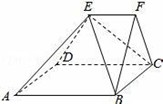
\includegraphics[width=0.3\linewidth]{Omega.16.jpg}
        \hspace{1cm} % 可选：图片右侧保留1cm间距（
    \end{figure}
    \newpage
    
    \item （本小题13分）
    
     在$\triangle ABC$中，内角$A,B,C$的对边分别为$a,b,c$，$c=1$。$\sqrt3 (a^2 \cos B \sin B + b^2 \cos A \sin A）=2\sin A \sin B$.
    \begin{enumerate}[label=(\Roman*)]
        \item 若$C$为锐角，求$C$；
        \item 若$a>b$,再从条件\textcircled {1}、条件\textcircled {2}、条件\textcircled {3}中选择一个作为已知，使得$\triangle ABC$存在且唯一，求$\triangle ABC$的周长.\\
        条件\textcircled {1}：$b=2$；\\
        条件\textcircled {2}：$BC$边上的高线长度是$\dfrac{1}{2}$;\\
        条件\textcircled {3}：$AB$边上的角平分线长度为$\dfrac{2}{3}$.\\
        注：如果选择的条件不符合要求，第$(2)$问得$0$分；如果选择多个符合要求的条件分别解答，按第一个解答计分.
    \end{enumerate}
    \newpage
    
    \item （本小题13分）
    
    某校进行二模考试时，按照以下规则来排考场座位：\\
    \textcircled {1}共有$8$个考场，每个考场共有$36$个座位。第$x$考场的第$y$座位表示为$(x,y)$；\\
    \textcircled {2}在一个考场内，座位序号按照蛇形，从小到大排列（如右下图）；\\
    \textcircled {3}主科考试（语数外）的考场排布按照一模考试的总分名次从高到低依次排列。如：第$1$名在$(1,1)$，第$36$名在$(1,36)$，第$37$名在$(2,1)$，第$74$名在$(3,3) \ldots$\\
    \textcircled {4}选科考试的考场排布按照一模考试赋分从高到低依次排列。同一赋分内随机分布.
    \begin{enumerate}[label=(\Roman*)]
        \item $A$与$B$一模总分相差$12$名，则求$A$与$B$在同一考场的概率;
        \item $A$与$B$都选地理，且一模考试中$A$赋了$100$分，$B$赋了$97$分。若该校一模地理共有$3$人赋$100$分，共有$9$人赋$97$分，且$A$与$B$座位在同一列。设$A$与$B$之间的距离为$X$，求$X$的分布列和期望;（定义距离为两个人座位序号之差的绝对值）
        \item $M,N,P,Q$四个人都选化学，且一模考试中$M,N$都赋了$88$分，$P,Q$都赋了$85$分。已知该校一模赋分在$88$分以上的有$26$人，赋分为$88$的有$9$人，赋分$85$的有$13$人。设$M$与$N$为同桌的概率为$P_1$，$P$与$Q$为同桌的概率为$P_2$，直接写出$P_1$与$P_2$的大小关系.\\
    \end{enumerate}

    \hfill
    \begin{tabular}{|c|c|c|c|c|c|}
        \hline
        36 & 25 & 24 & 13 & 12 & 1 \\
        \hline
        35 & 26 & 23 & 14 & 11 & 2 \\
        \hline
        34 & 27 & 22 & 15 & 10 & 3 \\
        \hline
        33 & 28 & 21 & 16 & 9 & 4 \\
        \hline
        32 & 29 & 20 & 17 & 8 & 5 \\
        \hline
        31 & 30 & 19 & 18 & 7 & 6 \\
        \hline
    \end{tabular}
    \newpage
    
    \item （本小题15分）
    
    已知$E$：$\dfrac{x^2}{a^2}+\dfrac{y^2}{b^2}=1\ (a>b>0)$的离心率为$\dfrac{1}{2}$，点$A(2,0)$和点$P(x_0,y_0)$在椭圆上.
    \begin{enumerate}[label=(\Roman*)]
        \item 求椭圆E的方程;
        \item 设$O$为原点，$Q$为$AP$中点。若点$P$位于第一象限，$P$关于$x$轴对称点为$P_1$，直线$x_0x-4y_0y=4$与直线$OP$交于$M$，设$\triangle OMP_1$与$\triangle OQP$的面积为$S_1,S_2$，求$\dfrac{S_1}{S_2}$.
    \end{enumerate}

    \vspace*{\fill}
    \item （本小题15分）
    
    设函数$f(x)=ax\ln x-x^2+1\ (a \ge 0)$.
    \begin{enumerate}[label=(\Roman*)]
        \item 若$a=2$，求函数$y=f(x)$ 在$(1,f(1))$处的切线方程;
        \item 若$f(x)(x-1) \le 0$恒成立，求$a$的取值范围;
        \item 若$f(x)$存在极小值点$x_1$和极大值点$x_2$，若$x_1 x_2<t$恒成立，求$t$的取值范围.
    \end{enumerate}
    \vspace*{\fill}
    
\end{enumerate}

% ============== 知己知彼Omega参考答案 ===============
\clearpage %新的一页
\setcounter{enumi}{0}   % 题号从1开始
\phantomsection
\addcontentsline{toc}{section}{参考答案} %加入目录
\setcounter{chapPage}{1} %初始化页数
\fancyfoot[C]{\small 第 \thechapPage 页 /共$1$页} %居中页脚

\begin{center} 
    {\LARGE \textbf{参考答案}}\\[1em]
\end{center}

\sectiontitle{一、选择题（共 $10$ 小题，每小题 $4$ 分，共 $40$ 分）}

    \begin{tasks}[label=(\arabic*), after-item-skip=0.6em,start=1] (5)
        \task $B$ 
        \task $C$
        \task $A$
        \task $D$        
        \task $B$
        \task $B$        
        \task $D$
        \task $B$        
        \task $D$
        \task $C$
    \end{tasks}

\sectiontitle{二、填空题（共5小题，每小题5分，共25分）}

    \begin{tasks}[label=(\arabic*), after-item-skip=0.6em,start=11] (2)
        \task $-540$ 
        \task $\dfrac{136 \sqrt{3} }{625}$
        \task $5 \pi$
        \task 答案不限，$(\ 2,+\infty\ )$        
        \task \textcircled{2} \textcircled{4}
    \end{tasks}

\sectiontitle{三.解答题（共6小题，共85分）}

    \begin{tasks}[label=(\arabic*), after-item-skip=0.6em,start=16] (1)
        \task 
        (I) (i) \ $5$\\[0.6em]
        (II) \ $-\dfrac{4}{5}$、$4$ \\

        \task
        (I)\ $\dfrac{\pi}{3}$\\[0.6em]
        (II)\ 只能选\textcircled{3}，$3+\sqrt{3}$ \\

        \task
        (I)\ $\dfrac{1}{3}$ \\[0.6em]
        (II)\ $EX=3$\\[0.6em]
        (III)\ $P_1>P_2$\\

        \task
        (I)\ $\dfrac{x^2}{4}+y^2= 1$ \\[0.6em]
        (II)\ $\dfrac{1}{4}$\\
        
        \task
        (I)\ $y=0$\\[0.6em]
        (II)\ $2$\\[0.6em]
        (III)\ $(\ 0,+\infty\ )$
    
    \end{tasks}

%================= 知己知彼51 ===================
\newpage
\phantomsection
\addcontentsline{toc}{section}{\texorpdfstring{知己知彼$51$}{知己知彼51}} % 加入目录
\setcounter{chapPage}{1} %初始化页数
\fancyfoot[C]{\small 高三数学\ 第 \thechapPage 页 (共$8$页)} %居中页脚

\begin{center}%标题
    {\LARGE \textbf{知己知彼$51$}}\\[1em]
\end{center}

\sectiontitle{一、选择题共 $10$ 小题，每小题 $4$ 分，共 $40$ 分。在每小题的四个选项中，选出符合题目要求的一项。}

\begin{enumerate}

    \item 设集合$M=\{x \mid x=2k+1\ ,\ k \in \mathbb{Z}\}$,$N=\{x\mid x=3k-1\ ,\ k \in \mathbb{Z}\}$，则$M\ \cap\ N=$
    \begin{tasks}(2)
        \task $\{x \mid x=2k+1\ ,\ k \in \mathbb{Z}\}$
        \task $\{x \mid x=3k-1\ ,\ k \in \mathbb{Z}\}$
        \task $\{x \mid x=6k+1\ ,\ k \in \mathbb{Z}\}$
        \task $\{x \mid x=6k-1\ ,\ k \in \mathbb{Z}\}$
    \end{tasks}

    \item 已知 $3+i$ 是关于 $x$ 的方程 $2x^2-mx+n=0 \ (m,n \in \mathbb{R})$ 的一个根，则 $m+n=$
    \begin{tasks}(4)
        \task $20$ 
        \task $22$
        \task $30$
        \task $32$
    \end{tasks}

    \item 要得到函数 $y= (\dfrac{1}{2})^{2x-1}$的图像，只需将指数函数$y=(\dfrac{1}{4})^{x}$的图像
    \begin{tasks}(2)
        \task 向左平移$1$个单位 
        \task 向右平移$1$个单位 
        \task 向左平移$\dfrac{1}{2}$个单位 
        \task 向右平移$\dfrac{1}{2}$个单位 
    \end{tasks}

    \item 下列关于函数$y=f(x)$和$y=f(2x-1)$的叙述中，错误的是
    \begin{enumerate}[label=(\Alph*)]
        \item 若$y=f(x)$的定义域是$\mathbb{R}$,则$y=f(2x-1)$的定义域是$\mathbb{R}$
        \item 若$y=f(x)$的值域是$(\ 0\ ,\ +\infty \ )$，则$y=f(2x-1)$的值域是$(\ 0\ ,\ +\infty \ )$
        \item 若$y=f(x)$在区间$(\ -1\ ,\ 1 \ )$上单调递增，则$y=f(2x-1)$在区间$(\ -1\ ,\ 1 \ )$上单调递增
        \item 若函数$y=f(2x-1)$是偶函数，则$y=f(x)$的图像关于$x=-1$对称
    \end{enumerate}
    \newpage
    
    \item 设$\aleph$为钝角 $v$ (单位： $km/s$ )，燃料质量 $M$ (单位： $kg$ )，与除燃料外的火箭质量$N$ (单位： $kg$ )满足：$v=2In(1+\dfrac{M}{N})$。若火箭燃料提供的最大速度约为 $16km/s$ ，则下列数值中与火箭发射时$\frac{M}{N}$最接近的是 （参考数据：$e \approx 2.7$，$\sqrt{30} \approx 5.4$）
    \begin{tasks}(4)
        \task $2000$ 
        \task $2500$
        \task $3000$
        \task $3500$
    \end{tasks}

    \item 设函数$f(x)= \sin (\omega x+ \phi)\  (\omega  > 0,\ 0 < \phi < \frac{\pi}{2})$，$f (\dfrac{5}{16}) = 0$，$f(x)$在$x= －\dfrac{1}{4}$处取得最小值，且$[\ \dfrac{1}{2}\ ,\ \dfrac{3}{4}\ ]$是$f(x)$的一个增区间，则$ \omega =$
    \begin{tasks}(4)
        \task $\dfrac{8\pi}{9}$ 
        \task $\dfrac{8\pi}{3}$
        \task $\dfrac{40\pi}{9}$
        \task 以上都不对
    \end{tasks}

    \item 一个不透明盒子中有 $3$ 个相同的球，其中有 $2$ 个橙球，$1$ 个白球。甲和乙两个人会从中抽 $2$ 个球并记录抽出球的颜色，其中甲每抽完一个球就放回去，乙抽完球不放回。
    设甲抽出的橙球数量为$X$ ，$X$ 的期望为 $E(X)$，方差为$D(X)$；乙抽出的橙球量数为$Y$ ，$Y$的期望为$E(Y)$，方差为$D(Y)$。则下列说法正确的是  
    \begin{enumerate}[label=(\Alph*)]
        \item $E(X)>E(Y)$，$D(X)=D(Y)$
        \item $E(X)=E(Y)$，$D(X)<D(Y)$
        \item $E(X)=E(Y)$，$D(X)=D(Y)$
        \item $E(X)=E(Y)$，$D(X)>D(Y)$
    \end{enumerate}
    
\newpage
    \item 已知椭圆$E1$：$\dfrac{x^2}{a^2}+\dfrac{y^2}{b^2}=1$与双曲线$E2$：$\dfrac{y^2}{a^2}-\dfrac{x^2}{b^2}=1\ (a \neq b \neq 0)$，$O$为坐标轴原点，则下列说法正确的个数是\\
        \textcircled{1} $E1$ 与 $E2$ 可能有$0$、$2$或$4$个交点\\
        \textcircled{2} "$E1$ 与 $E2$无交点”的充要条件是“$a>b>0$”\\
        \textcircled{3} 若$E1$ 与 $E2$有四个交点$A,B,C,D$分别位于第一、二、三、四象限，$\triangle ABO$为等边三角形，则$E2$ 与 $E1$离心率之比为$\sqrt6$
    \begin{tasks}(4)
        \task $0$ 个
        \task $1$ 个
        \task $2$ 个
        \task $3$ 个
    \end{tasks}

    \item  已知三棱锥$P-ABC$ 中，$Q$ 为 $PC$ 中点，$D$ 为$AC$ 中点，$PB\perp AB$ ，$QB=2$ ，$PA=2\sqrt2$， $BC=\sqrt3$，$cos \angle  QDB=－\dfrac{\sqrt2}{4}$，$\triangle ABC$的周长为$3+\sqrt3$，则 $PC$与面$ABC$夹角余弦值为
    \begin{tasks}(4)
        \task $\dfrac{\sqrt2}{2}$ 
        \task $\dfrac{\sqrt 3}{2}$
        \task $\dfrac{\sqrt6}{3}$
        \task 以上都不对
    \end{tasks}

    \item 数学课上，老师给出了曲线$E$的表达式：$f(\sin 2x)=\sin x$，对于$f(x)$是否为一个函数，同学们产生了质疑，则下列说法正确的是
    \begin{enumerate}[label=(\Alph*)]
        \item 取$x=\dfrac{\pi}{4}$和$x=\dfrac{3\pi}{4}$能够证明$f(x)$不是函数
        \item 若$\sin x_1=\sin x_2$，$\sin (2x_1) \neq \sin (2x_2)$有解，则不能证明$f(x)$不是函数
        \item 设$y=\sin x$，$t=\sin (2x)$，则曲线$E$满足$t^2+(2y^2-1)^2=1$
        \item 设$y=\sin x$，$t=\sin (2x)$，则曲线$E$满足$y^2+(2t^2-1)^2=1$
    \end{enumerate}
\end{enumerate}

\vfill

\end{document}